\documentclass[border=4pt,tikz]{standalone}
\usepackage[T1]{fontenc}
\usepackage{lmodern}
\usetikzlibrary{positioning,arrows.meta,calc,fit,backgrounds,patterns}
% Shared visual language for the paper's architecture diagrams.
% Every fill differs in lightness, so the diagrams stay legible when printed
% in grayscale; colour is only a redundant cue.
\definecolor{ink}{HTML}{1B2A3A}
\definecolor{navyfill}{HTML}{D5E0EC}
\definecolor{navyedge}{HTML}{2F5D8A}
\definecolor{tealfill}{HTML}{BFD8D5}
\definecolor{tealedge}{HTML}{2A6F6C}
\definecolor{amberfill}{HTML}{F1DCAE}
\definecolor{amberedge}{HTML}{9C6512}
\definecolor{greyfill}{HTML}{E5E7EB}
\definecolor{greymid}{HTML}{8B939E}
\definecolor{redfill}{HTML}{F0CBC5}
\definecolor{rededge}{HTML}{9E3B32}

\tikzset{
  >={Stealth[length=2.0mm,width=1.5mm]},
  every node/.style={font=\footnotesize, text=ink},
  box/.style={draw=ink, line width=0.5pt, rounded corners=1.5pt,
              fill=greyfill, align=center, inner sep=3pt, minimum height=7mm},
  databox/.style={box, fill=amberfill, draw=amberedge},
  procbox/.style={box, fill=navyfill, draw=navyedge},
  repbox/.style={box, fill=tealfill, draw=tealedge},
  evalbox/.style={box, fill=redfill, draw=rededge},
  fadebox/.style={box, fill=white, draw=greymid, dashed},
  arr/.style={->, draw=ink, line width=0.6pt},
  darr/.style={->, draw=greymid, line width=0.6pt, dashed},
  lbl/.style={font=\scriptsize, text=ink, inner sep=1pt, fill=white, fill opacity=0.85, text opacity=1},
  note/.style={font=\scriptsize, text=ink, align=left, inner sep=1pt},
  badge/.style={draw=rededge, fill=redfill, rounded corners=6pt,
                font=\scriptsize\bfseries, text=rededge, inner sep=2.2pt},
  badgefrz/.style={draw=tealedge, fill=tealfill, rounded corners=6pt,
                font=\scriptsize\bfseries, text=tealedge, inner sep=2.2pt},
  group/.style={draw=greymid, line width=0.5pt, rounded corners=3pt, inner sep=6pt},
}


% NOTE: no brace group around multi-line node text (see fig_pipeline.tex).
\begin{document}
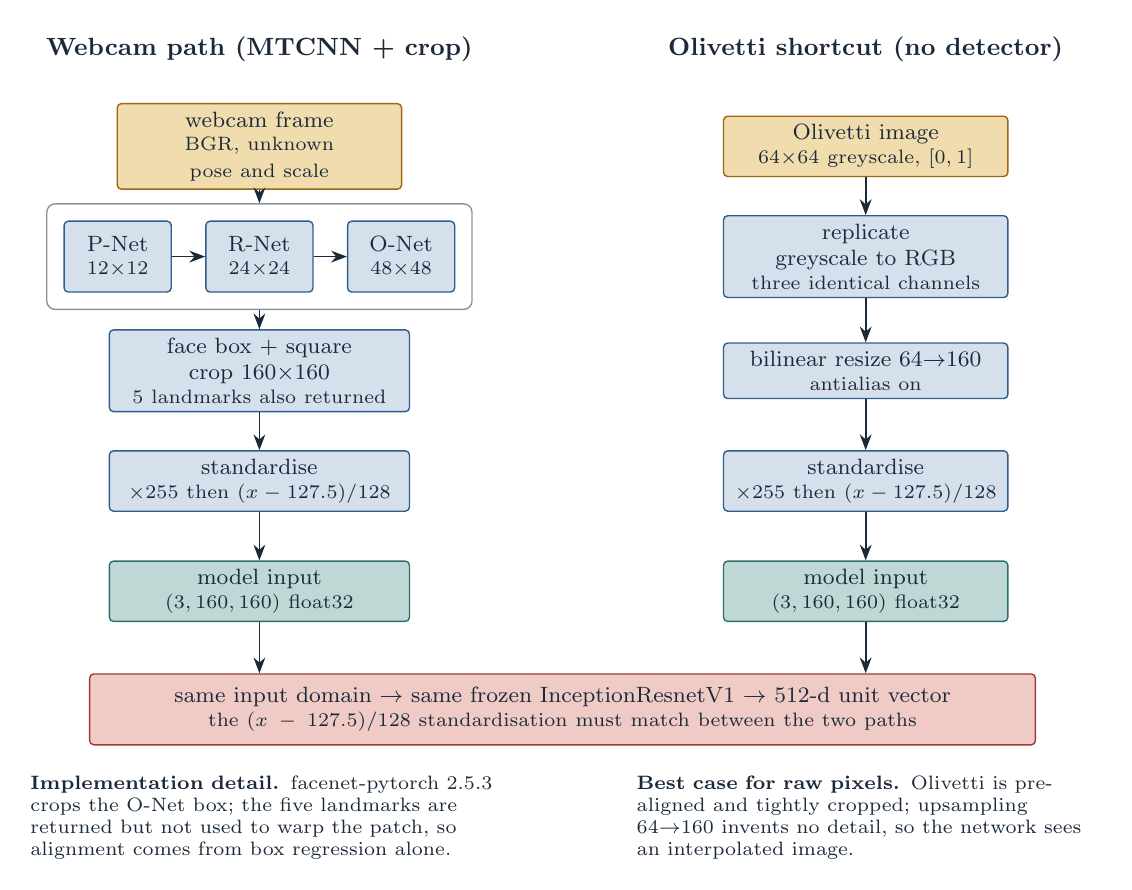
\begin{tikzpicture}[x=1cm,y=1cm]

% =================================================================== LEFT PANEL
\begin{scope}
  \node[font=\small\bfseries, anchor=south] at (3.3,5.75) {Webcam path (MTCNN + crop)};
  \node[databox, text width=3.4cm] (frame) at (3.3,4.80)
    {webcam frame\\[-1pt] \scriptsize BGR, unknown pose and scale};

  % MTCNN cascade container
  \node[procbox, text width=1.15cm, minimum height=9mm] (pnet) at (1.50,3.40)
    {P-Net\\[-1pt] \scriptsize 12$\times$12};
  \node[procbox, text width=1.15cm, minimum height=9mm] (rnet) at (3.30,3.40)
    {R-Net\\[-1pt] \scriptsize 24$\times$24};
  \node[procbox, text width=1.15cm, minimum height=9mm] (onet) at (5.10,3.40)
    {O-Net\\[-1pt] \scriptsize 48$\times$48};
  \begin{scope}[on background layer]
    \node[group, fit=(pnet)(onet)] (cascade) {};
  \end{scope}
  \draw[arr] (pnet) -- (rnet);
  \draw[arr] (rnet) -- (onet);

  \node[procbox, text width=3.6cm] (crop) at (3.3,1.95)
    {face box + square crop 160$\times$160\\[-1pt] \scriptsize 5 landmarks also returned};
  \node[procbox, text width=3.6cm] (std) at (3.3,0.55)
    {standardise\\[-1pt] \scriptsize $\times 255$ then $(x-127.5)/128$};
  \node[repbox, text width=3.6cm] (tensorA) at (3.3,-0.85)
    {model input\\[-1pt] \scriptsize $(3,160,160)$ float32};

  \draw[arr] (frame.south) -- (cascade.north);
  \draw[arr] (cascade.south) -- (crop.north);
  \draw[arr] (crop) -- (std);
  \draw[arr] (std) -- (tensorA);
\end{scope}

% =================================================================== RIGHT PANEL
\begin{scope}
  \node[font=\small\bfseries, anchor=south] at (11.0,5.75) {Olivetti shortcut (no detector)};
  \node[databox, text width=3.4cm] (olivimg) at (11.0,4.80)
    {Olivetti image\\[-1pt] \scriptsize 64$\times$64 greyscale, $[0,1]$};
  \node[procbox, text width=3.4cm] (repl) at (11.0,3.40)
    {replicate greyscale to RGB\\[-1pt] \scriptsize three identical channels};
  \node[procbox, text width=3.4cm] (resize) at (11.0,1.95)
    {bilinear resize 64$\to$160\\[-1pt] \scriptsize antialias on};
  \node[procbox, text width=3.4cm] (std2) at (11.0,0.55)
    {standardise\\[-1pt] \scriptsize $\times 255$ then $(x-127.5)/128$};
  \node[repbox, text width=3.4cm] (tensorB) at (11.0,-0.85)
    {model input\\[-1pt] \scriptsize $(3,160,160)$ float32};

  \draw[arr] (olivimg) -- (repl);
  \draw[arr] (repl) -- (resize);
  \draw[arr] (resize) -- (std2);
  \draw[arr] (std2) -- (tensorB);
\end{scope}

% =================================================================== SHARED END
\node[evalbox, text width=11.8cm, minimum height=9mm] (shared) at (7.15,-2.35)
  {same input domain $\rightarrow$ same frozen InceptionResnetV1 $\rightarrow$ 512-d unit vector\\[-1pt]
   \scriptsize the $(x-127.5)/128$ standardisation must match between the two paths};

\draw[arr] (tensorA.south) -- (tensorA.south |- shared.north);
\draw[arr] (tensorB.south) -- (tensorB.south |- shared.north);

% =================================================================== NOTES
\node[note, anchor=north west, text width=5.9cm] at (0.35,-3.15)
  {\textbf{Implementation detail.} facenet-pytorch 2.5.3 crops the O-Net box; the five landmarks are
   returned but not used to warp the patch, so alignment comes from box regression alone.};
\node[note, anchor=north west, text width=5.9cm] at (8.05,-3.15)
  {\textbf{Best case for raw pixels.} Olivetti is pre-aligned and tightly cropped; upsampling
   64$\to$160 invents no detail, so the network sees an interpolated image.};

\end{tikzpicture}
\end{document}
